% Kapitel 4: Ergebnisse
\section{Ergebnisse}
\label{sec:ergebnisse}

Dieses Kapitel präsentiert die Ergebnisse der Simulationsexperimente. Der Aufbau folgt den zentralen Fragen der Arbeit: Zunächst geht es um den Einfluss der Topologie, dann um den Unterschied zwischen zufälligen und gezielten Störungen, und schließlich um die Besonderheiten der Interdependenz im Smart Grid.

Alle Experimente wurden mit $N = 500$ Knoten durchgeführt, jeweils 30 unabhängige Läufe pro Konfiguration, bei einer Schrittweite von 5\,\%. Als zentrale Metrik dient die AUC, ergänzt durch die Visualisierung der Robustheitskurven.

\subsection{Übersicht der Experimente}

Bevor es ins Detail geht, hier zunächst ein Überblick über die durchgeführten Experimente. Die Bezeichnungen F1 bis F6 werden im Folgenden durchgängig verwendet.

\begin{table}[H]
\centering
\caption{Übersicht der durchgeführten Experimente}
\label{tab:experimente}
\begin{tabular}{llllccc}
\hline
\textbf{ID} & \textbf{Modus} & \textbf{GP} & \textbf{Szenario} & \textbf{q} & \textbf{r} & \textbf{Korr.} \\
\hline
F1 & Konventionell & ER & Random (GP) & -- & -- & -- \\
F2 & Konventionell & BA & Random (GP) & -- & -- & -- \\
F3 & Konventionell & BA & Targeted (GP) & -- & -- & -- \\
F4 & Smart Grid & BA/BA & Targeted (GC) & 1.0 & 1 & Nein \\
F5 & Smart Grid & BA/BA & Targeted (GC) & 1.0 & 1 & Ja \\
F6 & Smart Grid & ER/ER & Targeted (GC) & 1.0 & 2 & Nein \\
\hline
\end{tabular}
\end{table}

\subsection{Topologieeffekt: ER vs. BA bei zufälligen Ausfällen}

Die erste Frage ist, ob die Topologie des Netzes einen Unterschied macht. Dazu vergleichen wir ein homogenes Erdős-Rényi-Netz (F1) mit einem skalenfreien Barabási-Albert-Netz (F2), beide unter zufälligen Ausfällen.

\begin{table}[H]
\centering
\caption{AUC bei zufälligen Ausfällen: ER vs. BA}
\label{tab:topologie}
\begin{tabular}{lcc}
\hline
\textbf{Experiment} & \textbf{AUC} & \textbf{Std} \\
\hline
F1: ER, Random & $0{,}953$ & $\pm 0{,}012$ \\
F2: BA, Random & $0{,}757$ & $\pm 0{,}037$ \\
\hline
\textbf{Differenz} & \multicolumn{2}{c}{$\Delta = 0{,}196$} \\
\hline
\end{tabular}
\end{table}

Das Ergebnis ist deutlich. Das ER-Netz behält bei zufälligen Ausfällen fast durchgehend seine Konnektivität, mit einer AUC von knapp 0,95. Das BA-Netz kommt nur auf 0,76. Die Differenz von fast 0,2 ist erheblich.

Warum ist das so? Bei einem ER-Netz sind die Grade relativ gleichmäßig verteilt. Jeder Knoten hat ungefähr gleich viele Verbindungen. Wenn man zufällig Knoten entfernt, trifft man meistens ''normale'' Knoten, und das Netz bleibt zusammen. Beim BA-Netz gibt es dagegen einige wenige Hubs mit sehr vielen Verbindungen. Obwohl man beim zufälligen Entfernen mit hoher Wahrscheinlichkeit \textit{nicht} die Hubs trifft, reicht die heterogene Struktur aus, um das Netz insgesamt fragiler zu machen.

\begin{figure}[H]
    \centering
    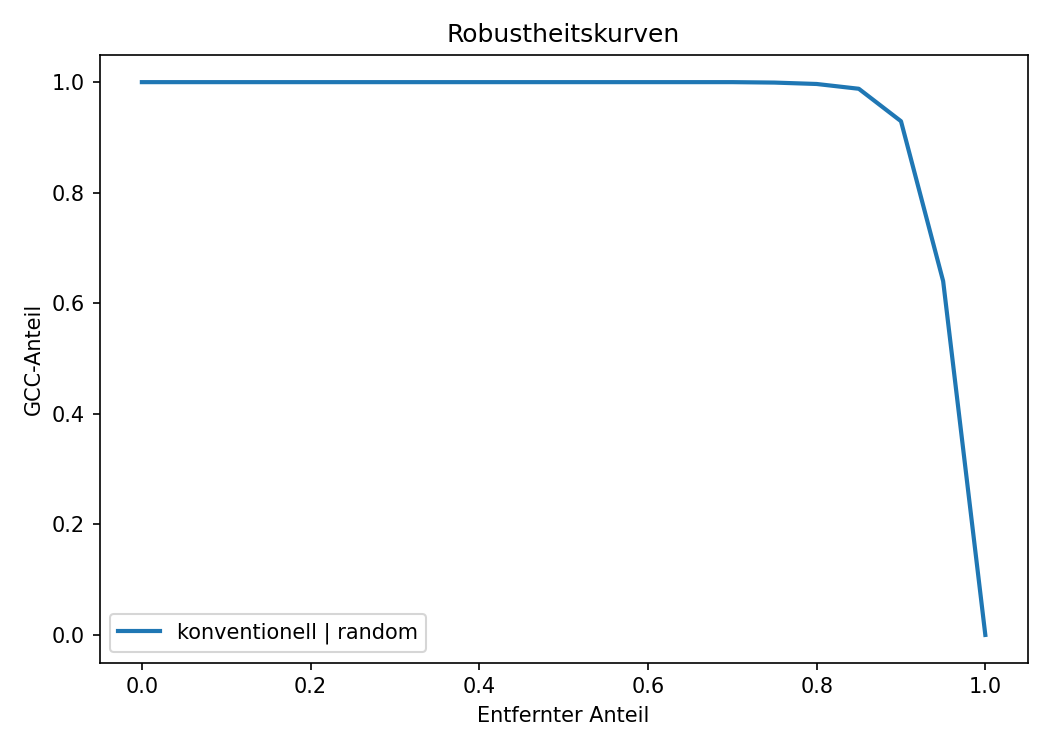
\includegraphics[width=0.75\textwidth]{figures/F1_baseline_er_random.png}
    \caption{Robustheitskurve des ER-Netzes bei zufälligen Ausfällen (F1). Das Netz bleibt bis etwa 60\,\% Knotenentfernung weitgehend intakt.}
    \label{fig:f1_er_random}
\end{figure}

\begin{figure}[H]
    \centering
    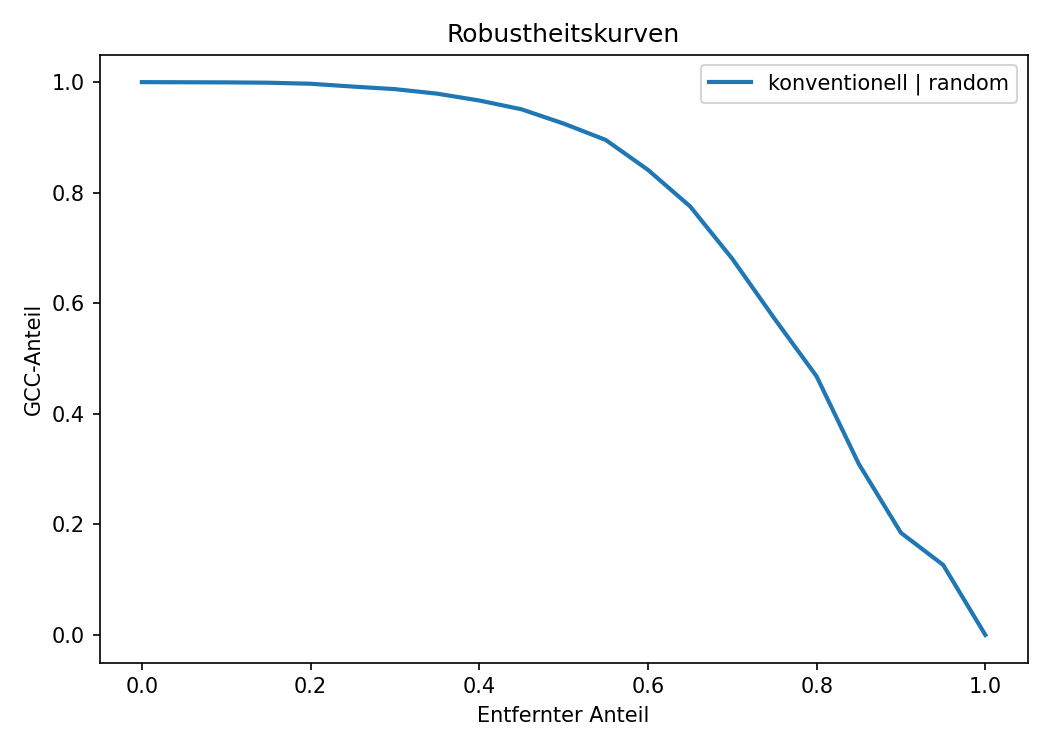
\includegraphics[width=0.75\textwidth]{figures/F2_baseline_ba_random.png}
    \caption{Robustheitskurve des BA-Netzes bei zufälligen Ausfällen (F2). Der Abfall beginnt früher und verläuft steiler als beim ER-Netz.}
    \label{fig:f2_ba_random}
\end{figure}

\subsection{Zufällig vs. Gezielt: Der Unterschied macht sich bemerkbar}

Jetzt wird es interessant. Was passiert, wenn man nicht zufällig angreift, sondern gezielt die wichtigsten Knoten ausschaltet? Für diesen Vergleich bleiben wir beim BA-Netz und stellen F2 (zufällig) neben F3 (gezielt).

\begin{table}[H]
\centering
\caption{Vergleich: Zufällige vs. gezielte Angriffe auf ein BA-Netz}
\label{tab:random_vs_targeted}
\begin{tabular}{lcc}
\hline
\textbf{Experiment} & \textbf{AUC} & \textbf{Std} \\
\hline
F2: BA, Random & $0{,}757$ & $\pm 0{,}037$ \\
F3: BA, Targeted & $0{,}233$ & $\pm 0{,}011$ \\
\hline
\textbf{Differenz} & \multicolumn{2}{c}{$\Delta = 0{,}524$} \\
\hline
\end{tabular}
\end{table}

Der Unterschied ist dramatisch. Die AUC fällt von 0,76 auf 0,23 -- das entspricht einem Rückgang um mehr als zwei Drittel. Bei gezielten Angriffen bricht das BA-Netz praktisch zusammen.

Das ist die bekannte Achillesferse skalenfreier Netze: Sie sind robust gegen zufällige Ausfälle, weil die meisten Knoten unwichtig sind. Aber sie sind extrem verwundbar gegen gezielte Angriffe, weil wenige Hubs das ganze Netz zusammenhalten. Entfernt man diese Hubs gezielt, zerfällt das Netz sofort.

\begin{figure}[H]
    \centering
    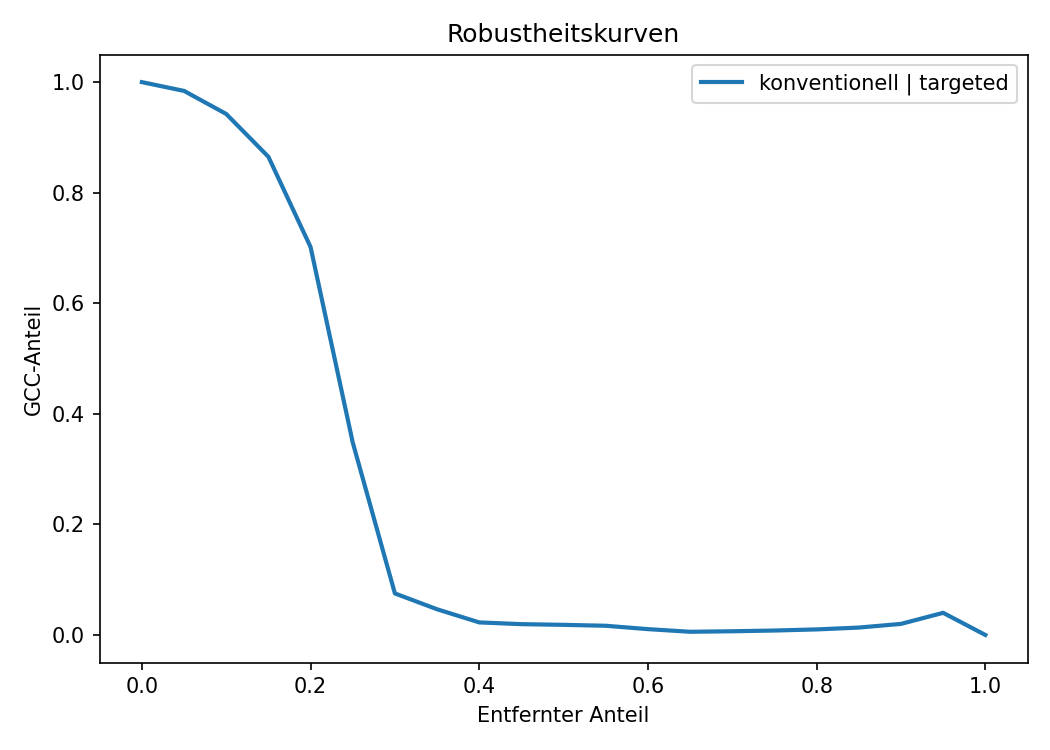
\includegraphics[width=0.75\textwidth]{figures/F3_baseline_ba_targeted.png}
    \caption{Robustheitskurve des BA-Netzes bei gezieltem Angriff (F3). Schon bei 10\,\% Knotenentfernung ist die GCC stark reduziert.}
    \label{fig:f3_ba_targeted}
\end{figure}

Die Kurve in Abbildung~\ref{fig:f3_ba_targeted} zeigt das eindrücklich. Bereits nach Entfernung von 10\,\% der Knoten ist die größte zusammenhängende Komponente auf einen Bruchteil geschrumpft. Das ist ein fundamentaler Unterschied zu den Kurven bei zufälligen Ausfällen.

\subsection{Interdependenz: Der Effekt der Kopplung}

Nun kommen wir zum eigentlichen Kern der Arbeit: Was ändert sich, wenn das Stromnetz mit einem Kommunikationsnetz gekoppelt ist? Und wie hängt der Effekt von der Struktur dieser Kopplung ab?

Für diesen Vergleich betrachten wir zwei Varianten: Bei F4 werden die Abhängigkeiten zufällig zugewiesen, bei F5 korreliert (wichtige Stromknoten hängen von wichtigen Kommunikationsknoten ab). Angegriffen wird in beiden Fällen das Kommunikationsnetz.

\begin{table}[H]
\centering
\caption{Einfluss der Abhängigkeitsstruktur bei Angriff auf das Kommunikationsnetz}
\label{tab:interdependenz}
\begin{tabular}{lcc}
\hline
\textbf{Experiment} & \textbf{AUC} & \textbf{Std} \\
\hline
F4: Zufällige Abhängigkeiten & $0{,}739$ & $\pm 0{,}041$ \\
F5: Korrelierte Abhängigkeiten & $0{,}233$ & $\pm 0{,}011$ \\
\hline
\textbf{Differenz} & \multicolumn{2}{c}{$\Delta = 0{,}506$} \\
\hline
\end{tabular}
\end{table}

Das Ergebnis ist bemerkenswert. Bei zufälliger Zuweisung bleibt das System trotz vollständiger Kopplung ($q = 1$) relativ robust. Die AUC von 0,74 ist vergleichbar mit dem BA-Netz unter zufälligen Ausfällen. Der Angriff auf das Kommunikationsnetz propagiert zwar ins Stromnetz, aber er trifft nicht systematisch die wichtigen Knoten.

Bei korrelierter Zuweisung kippt das Bild komplett. Die AUC sinkt auf 0,23 -- exakt der Wert, den wir bei einem direkten gezielten Angriff auf das Stromnetz gesehen haben (F3). Das ist kein Zufall. Bei korrelierter Kopplung bedeutet ein Angriff auf die Hubs des Kommunikationsnetzes automatisch auch den Ausfall der Hubs im Stromnetz.

\begin{figure}[H]
    \centering
    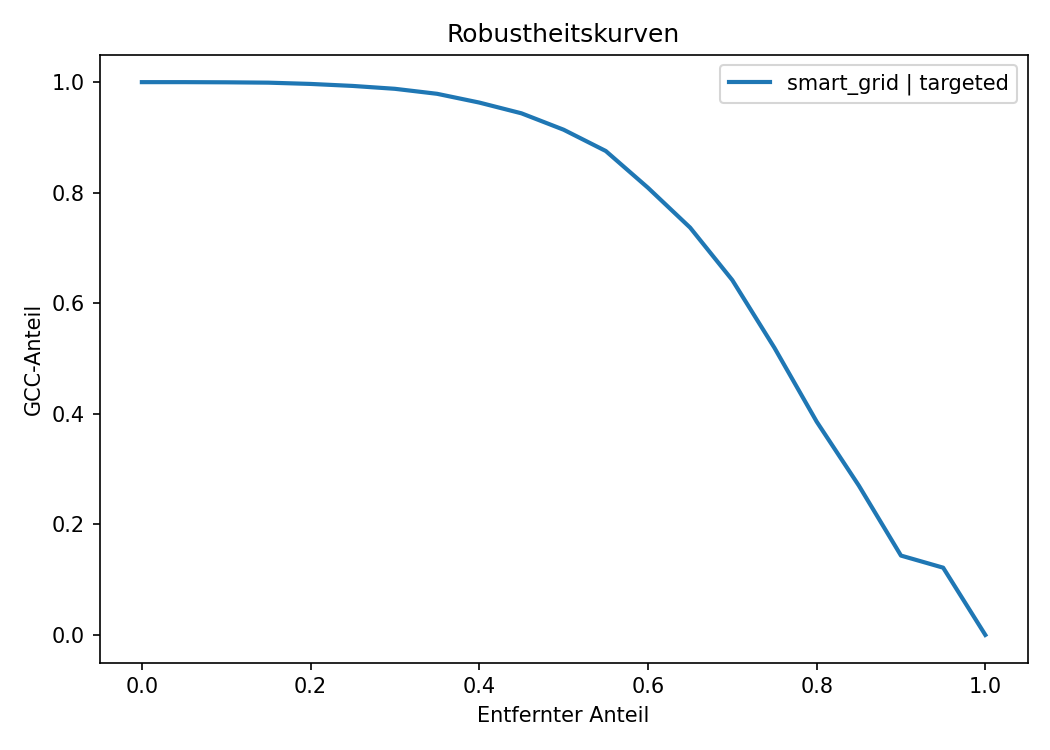
\includegraphics[width=0.75\textwidth]{figures/F4_smartgrid_random_deps.png}
    \caption{Smart Grid mit zufälligen Abhängigkeiten (F4). Der Angriff auf GC propagiert, aber das System bleibt vergleichsweise stabil.}
    \label{fig:f4_random_deps}
\end{figure}

\begin{figure}[H]
    \centering
    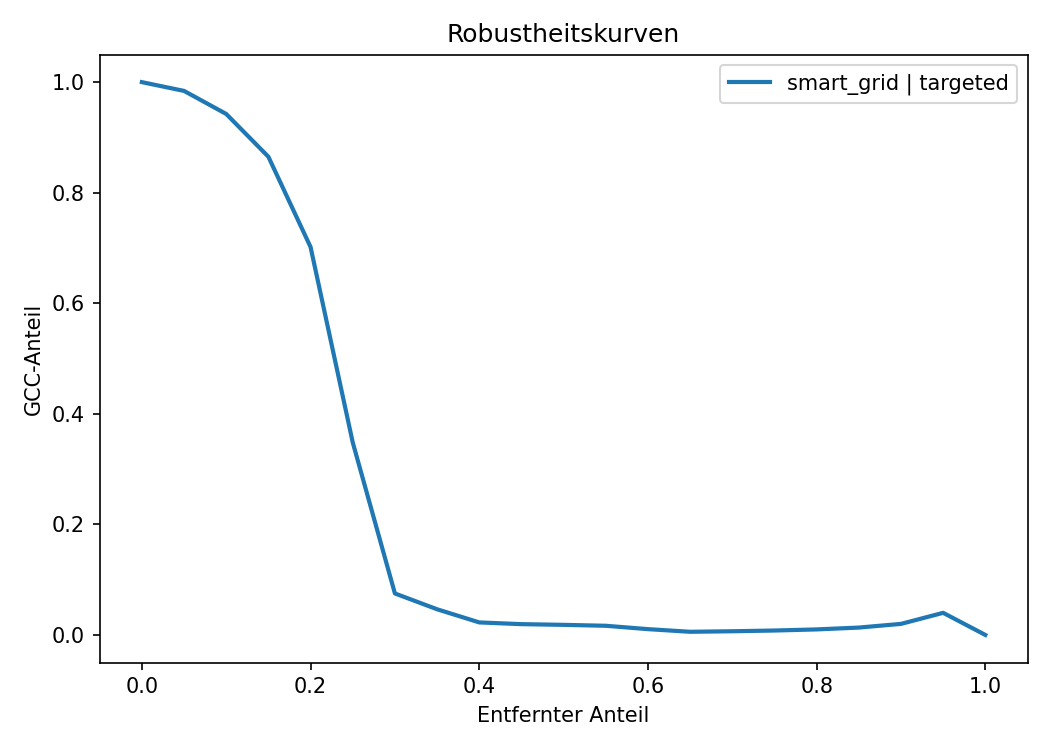
\includegraphics[width=0.75\textwidth]{figures/F5_smartgrid_correlated_deps.png}
    \caption{Smart Grid mit korrelierten Abhängigkeiten (F5). Der Kurvenverlauf entspricht dem eines direkten Angriffs auf das physische Netz.}
    \label{fig:f5_correlated_deps}
\end{figure}

Die Schlussfolgerung ist klar: Die bloße Existenz von Interdependenzen macht ein Netz noch nicht fragil. Entscheidend ist, \textit{wie} die Abhängigkeiten strukturiert sind.

\subsection{Redundanz als Schutzmaßnahme}

Ein naheliegender Ansatz zur Erhöhung der Robustheit ist Redundanz bei den Abhängigkeiten. Wenn ein Stromknoten von zwei statt einem Kommunikationsknoten abhängt, muss der Angreifer beide ausschalten, um den Stromknoten zu treffen. Experiment F6 testet genau das.

\begin{table}[H]
\centering
\caption{Schutzwirkung der Redundanz ($r = 2$)}
\label{tab:redundanz}
\begin{tabular}{lcc}
\hline
\textbf{Experiment} & \textbf{AUC} & \textbf{Std} \\
\hline
E5 (ER, q=1.0, r=1) & $0{,}886$ & $\pm 0{,}028$ \\
F6 (ER, q=1.0, r=2) & $0{,}970$ & $\pm 0{,}004$ \\
\hline
\textbf{Verbesserung} & \multicolumn{2}{c}{$+8{,}4\%$} \\
\hline
\end{tabular}
\end{table}

Die Redundanz wirkt. Mit $r = 2$ steigt die AUC auf 0,97 -- fast so hoch wie bei einem ungekoppelten ER-Netz. Die Streuung sinkt ebenfalls deutlich, was auf ein insgesamt stabileres Verhalten hindeutet.

\begin{figure}[H]
    \centering
    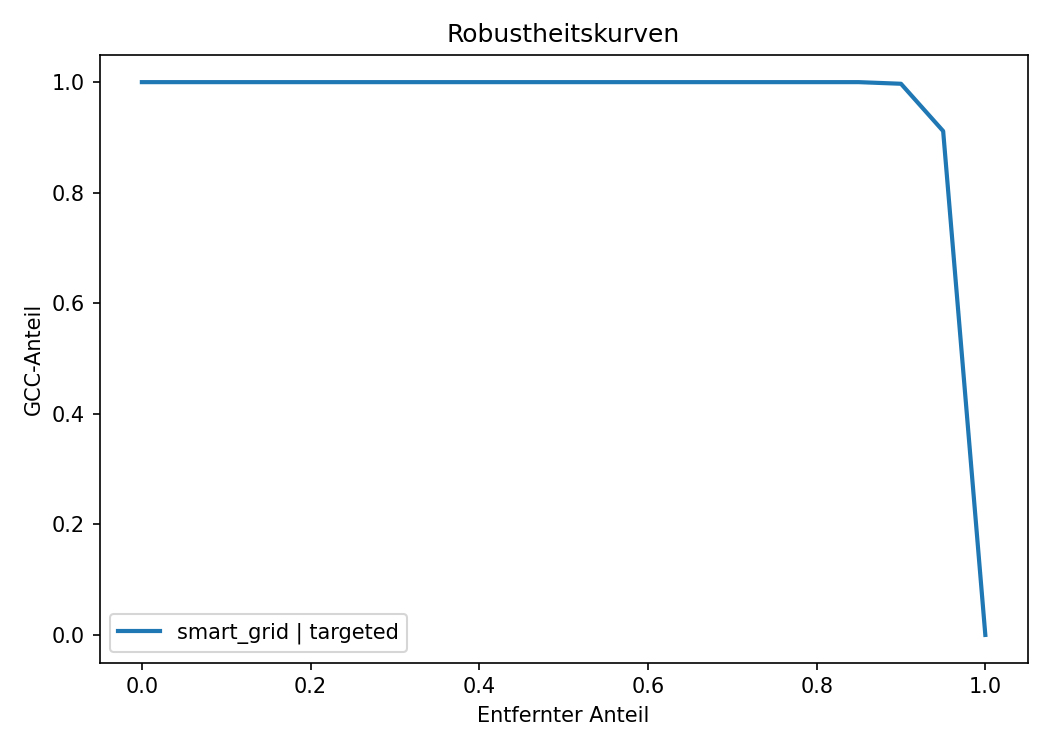
\includegraphics[width=0.75\textwidth]{figures/F6_smartgrid_redundanz.png}
    \caption{Smart Grid mit Redundanz $r = 2$ (F6). Das System bleibt über den gesamten Entfernungsbereich nahezu vollständig vernetzt.}
    \label{fig:f6_redundanz}
\end{figure}

Allerdings -- und das ist wichtig -- wurde F6 mit zufälliger Abhängigkeitszuweisung durchgeführt. Bei korrelierter Zuweisung, wo beide Abhängigkeiten eines Stromknotens wahrscheinlich ebenfalls an wichtige Kommunikationsknoten geknüpft sind, dürfte die Schutzwirkung geringer ausfallen. Das wäre ein Ansatzpunkt für weitere Untersuchungen.

\subsection{Zusammenfassung der Ergebnisse}

Tabelle~\ref{tab:zusammenfassung} fasst alle AUC-Werte zusammen.

\begin{table}[H]
\centering
\caption{Gesamtübersicht der AUC-Werte}
\label{tab:zusammenfassung}
\begin{tabular}{llc}
\hline
\textbf{ID} & \textbf{Beschreibung} & \textbf{AUC} \\
\hline
F1 & ER, Random auf GP & $0{,}953$ \\
F2 & BA, Random auf GP & $0{,}757$ \\
F3 & BA, Targeted auf GP & $0{,}233$ \\
F4 & Smart Grid, Random-Deps, Targeted auf GC & $0{,}739$ \\
F5 & Smart Grid, Korreliert, Targeted auf GC & $0{,}233$ \\
F6 & Smart Grid, ER, r=2, Targeted auf GC & $0{,}970$ \\
\hline
\end{tabular}
\end{table}

Drei Befunde stechen heraus:

\begin{enumerate}
    \item Skalenfreie Netze sind deutlich verwundbarer als homogene Netze, besonders bei gezielten Angriffen. Die Differenz in der AUC beträgt bis zu 0,52.
    
    \item Die Struktur der Interdependenz ist wichtiger als die bloße Tatsache, dass eine Kopplung existiert. Korrelierte Abhängigkeiten verstärken die Verwundbarkeit dramatisch.
    
    \item Redundanz bei den Abhängigkeitsbeziehungen kann das System stabilisieren -- zumindest bei zufälliger Zuweisung. Ob das auch bei korrelierter Struktur gilt, bleibt offen.
\end{enumerate}
